\documentclass[12pt,a4paper,openany]{book}
\newcommand\tab[1][1cm]{\hspace*{#1}}
\usepackage{array,amsmath,amsthm,amssymb,graphicx,hyperref,wrapfig,tabularx,mathptmx,anyfontsize,t1enc}
\graphicspath{ {./images/} }
\usepackage[left=1.2in,right=1.2in,top=1in,bottom=1in]{geometry}
%\usepackage[romanian]{babel}
\usepackage[english]{babel}
\usepackage{xcolor}
\usepackage{paralist}
\usepackage[printonlyused,withpage]{acronym}
\RequirePackage{hyphenat}
\usepackage{algorithmic, algorithm}
\usepackage[inline]{enumitem}
%\usepackage{...insert other packages here...}
\newtheorem{thm}{Theorem}[section]
\newtheorem{lem}[thm]{Lemma}
\theoremstyle{definition}
\newtheorem{defn}{Definition}[section]
\theoremstyle{remark}
\newtheorem{rem}{Remark}[section]
\newtheorem{exmp}{Example}[section]

\begin{document}
\sloppy

\thispagestyle{empty}
\begin{center}
\begin{figure}[h!]
\vspace{-20pt}
\begin{center}

\includegraphics[width=100pt]{FMI-03.png}
\end{center}
\end{figure}


{\large{\bf WEST UNIVERSITY OF TIMI\c SOARA

FACULTY OF MATHEMATICS AND COMPUTER SCIENCE

BACHELOR STUDY PROGRAM:  Computer Science in English }}

\vspace{120pt}
{\huge {\bf BACHELOR THESIS}}

\vspace{160pt}
\end{center}

{\large\noindent{\bf SUPERVISOR:
\hspace{172pt} GRADUATE: }

\noindent Lect. Dr. Mafteiu-Scai Liviu Octavian\hfill 
\noindent  Șova Dumitru Ștefan Andrei}

\vfill
\begin{center}
{\bf TIMI\c SOARA

2022}
\end{center}
\newpage
\thispagestyle{empty}
\begin{center}
{\large{\bf WEST UNIVERSITY OF TIMI\c SOARA
		
FACULTY OF MATHEMATICS AND COMPUTER SCIENCE
		
BACHELOR STUDY PROGRAM:  Computer Science in English}}

\vspace{200pt}
{\huge {\bf Data Manager }}

\vspace{153pt}
\end{center}

{\large\noindent{\bf SUPERVISOR:\hfill GRADUATE:}

\noindent Lect. Dr. Mafteiu-Scai Liviu Octavian\hfill
\noindent Șova Dumitru Ștefan Andrei}
 

\vfill
\begin{center}
{\bf TIMI\c SOARA

2022}
\end{center}

\newpage
\normalsize{}

\section*{Abstract} 
The addressed problem is comprised of the storage of an Android phone, the proposed thesis comprises an application that proposes a way for its users to save storage space with minimal input. 

The way this app is going to save up on storage space is by looking at specific file types that the user can filter through, as such, the app will ask the user for the required permissions to be able to scan the phone and detect said unnecessary data/ applications. The following options will be available for the user: the ability to delete the cache memory, the option to check if there are currently files/folders in the trash, and an option to empty it if the user wants to or not, the option to delete the leftover data of an application that has been deleted, the option to delete empty folders, archive files, and \ac{APK} files, and the option to check the list of applications of the user and see the last time the user accessed them, with the ability to go to the \ac{app} info and delete/disable them or leave them alone.

Such options represent the more hidden parts of data management, most users being unaware that their storage space is being drained by such files, forgetting about apps that they haven't used in a while, or simply forgetting to empty their trash folders.

Keywords: Android Studio, Kotlin, data, management, cache, cleaning, files, delete, XML, memory.
\newpage
\normalsize{}

\section*{Rezumat} 
Problema abordată constă în memoria unui telefon Android, lucrarea propusă cuprinde o aplicație ce propune utilizatorilor săi o modalitate de-a economisi spațiu de stocare cu un input minim.

Modul în care această aplicație va economisi spațiul de stocare este prin a analiza anumite tipuri de fișiere pe care utilizatorul le poate filtra, și, aplicația îi va cere acestuia permisiunile necesare pentru a putea scana telefonul și pentru a putea detecta respectivele fișiere inutile. Următoarele opțiuni vor fi disponibile pentru utilizatori: posibilitatea de a șterge memoria cache, opțiunea de a verifica dacă există în prezent fișiere/foldere în coșul de gunoi și o opțiune de-al goli dacă utilizatorul dorește sau nu, opțiunea de a șterge datele rămase ale unei aplicați care a fost dezinstalată, opțiunea de a șterge folderele goale, fișierele de arhivă și fișierele \ac{APK} și opțiunea de a verifica lista de aplicații ale utilizatorului și de a vedea ultima dată când acesta le-a accesat, cu posibilitatea de a accesa informațiile \ac{app} și de a le șterge/dezactiva sau de a le lăsa în pace.

Astfel de opțiuni reprezintă părțile mai ascunse ale gestionări datelor, majoritatea utilizatorilor neștiind că spațiul lor de stocare este epuizat de astfel de fișiere, uitând de aplicațiile pe care nu le-au folosit de ceva vreme sau pur și simplu uitând să își golească dosarul de gunoi.

Cuvinte cheie: Android Studio, Kotlin, date, gestionare, cache, curățare, fișiere, ștergere, XML, memorie.
\newpage
\normalsize{}

\tableofcontents
\listoffigures

% inline
{\noindent \huge \textbf{List of acronyms}\par}

\begin{acronym}
 \acro{UI}{User Interface}
 \acro{CPU}{Central processing unit}
 \acro{OS}{Operating System}
 \acro{GB}{Gigabytes}
 \acro{APK}{Android Package}
 \acro{app}{Application}
 \acro{MB}{Megabytes}
 \acro{IDE}{Integrated Development Environment}
 \acro{NDK}{Android Native Development Kit}
 \acro{p}{pixels}
 \acro{API}{Application programming interface}
 \acro{JSON}{JavaScript Object Notation}
 \acro{AI}{Artificial Inteligence}
 \acro{4K}{3840 x 2160 resolution}
\end{acronym}
%%%%%%%%%%%%%%%%%%%%%%%%%%%%%%%%%%%%%%%%%%%%%%%%%
%%%%%%%%%%%% cap: intro %%%%%%%%%%%%%%%%%
%%%%%%%%%%%%%%%%%%%%%%%%%%%%%%%%%%%%%%%%%%%%%%%%%

\chapter{Introduction}\label{cap:intro}

DataManager is designed with the users' phones' data management in the foreground, focusing on a simple interface that doesn't require much from the user, with options for emptying their trash, cleaning unneeded data, and being able to see what applications they have not used regularly, each done with one press of a button only.

The app offers different menus for each of its use cases, each with an easy-to-use and easy-to-understand layout. For further convenience, the app also offers the ability to enter a general settings menu where the user can change the overall theme of the app, from a light theme to a dark one, and to change the language from English to Romanian.

The three main screens of the app consist of the cache cleaning screen, the unused applications screen, and the main menu screen. The main menu gives access to the other screens, the option to empty the trash folder, and the general settings screen, where the user can change certain preferences about the application. The other two screens are for data management, the cache screen allows the user to select filters for what he wants to delete, and the unused applications screen lists the applications of the user and the last time they were used, with the option to delete them if he wished to.

For accessing the storage, internet, and so on, the application will ask the user for the required permissions. All permissions are described in a special menu found in the main menu that tells the user exactly what are they used for.

\newpage

\section{Motivation}\label{sect:Motivation}

\begin{wrapfigure}{r}{0.4\textwidth} 
    \centering
    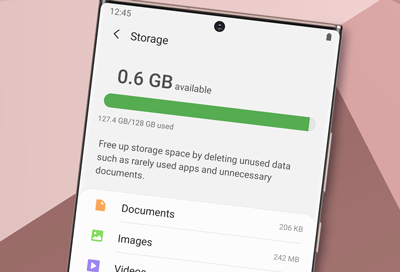
\includegraphics[width=0.4\textwidth]{storage.png}
    \caption{The common sight of an emptying storage}
    \label{fig:batteryImage}
\end{wrapfigure}

Owning a phone has become in the last decade a basic human need for all of us, regardless of age, culture, or background. The phone helps connect us with one another, not just by making phone calls or writing messages to one another, but modern phones also allow us to use the internet, share our stories, photos, life experiences, and so much more. Besides connecting with one another, it gives us countless possibilities, from entertaining us to educating us and so on. 

Owning to this fact, one of the most important factors of our phones, that we usually do not take into consideration or notice too late is the well-being of the phone, usually being represented by the neglect of our storage spaces. It is easy to lose track of our storage and find ourselves in the awkward situation of needing to take a picture, download a file for work, or just install the hottest new app, and being unable to do so because we are hit with the surprise of no more storage space left. Not only that, but one aspect of the phone that everybody seems to not pay attention to is the well-being of the phone, many forget to delete leftover data from uninstalled applications, empty the trash folder, and so on, little things that in time add up to a worse functioning phone and a smaller storage space.

Such unneeded files like caches, logs, \ac{APK} files, and so on, are the type of files that the user will never think about, and especially not think to clean up to save on his or her phone memory.

\section{Problem Statement}\label{sect:Problem Statement}

This problem becomes more and more prevalent with the size of newer applications, the increase in resolution for photos and videos, and the amount of data that remains from them. A simple 1080\ac{p} photo is around 6 \ac{MB}, while a phone with \ac{4K} capabilities is around 24 \ac{MB}, which is an increase of 4 times. Things are even worse when looking at video memory, a 1080\ac{p} 1-minute video has around 100 \ac{MB} while a \ac{4K} one has around 450 \ac{MB}.

With this in mind, every little amount of memory that the user can save up is usually more than welcomed, but unfortunately, phones do not come with built-in memory managers from the manufacturers.

As such, the problem of how to save our storage space for our phones usually remains in the hands of the consumer, usually by downloading a third-party application that gets the job done. 
\newpage

\section{Thesis Scope and Objectives}\label{sect:Thesis Scope and Objectives}

Possible solutions to such problems include the very functions of the proposed application, with how much we tend to use our phones in everyday life, too little time is spent taking care of them and managing their storage in a healthy manner.

The improvements will have certain liberties that the user will have to give his consent to, such as the functionality to access the external storage and usage for the application, however, such improvements will prove fruitful to those who want an increase in storage space, without the need for searching through every application for signs of residual data.

\section{Thesis Structure}\label{sect:Thesis Structure}

The thesis will have a format consisting of 5 main chapters, each with various sections, each chapter looking at a different aspect of the thesis. The 5 chapters are as follows:

    • The first chapter focuses on the what and the why of the project, sharing the motivation behind the project and a general overview behind it;

    • The second chapter looks at the application architecture, its main use cases, its main flow, and the expected app requirements;

    • Chapter 3 focuses on similar applications that are in the same genre as this thesis, looking at their varied utilities, and functions, and concluding at the end of the chapter with a comparison between them;

    • Chapter 4  looks at the implementation that was used for creating the application, and the methods and classes that were used;

    • The last chapter is the user manual for the application, guiding the user through each of the main screens, what they do, what permissions they require, and what setting options the user has access to;

After these chapters, the app will also have a chapter for conclusions and discussions based on the results, as well as a bibliography for users' reference.
%%%%%%%%%%%%%%%%%%%%%%%%%%%%%%%%%%%%%%%%%%%%%%%%%
%%%%%%%%%%%% chap: Related Work%%%%%%%%%%%%%%%%%
%%%%%%%%%%%%%%%%%%%%%%%%%%%%%%%%%%%%%%%%%%%%%%%%%

\chapter{Related Work}\label{chapter:chap3}

\section{Similar Applications}\label{sect:similar applications}

\begin{wrapfigure}{r}{0.4\textwidth} 
    \centering
    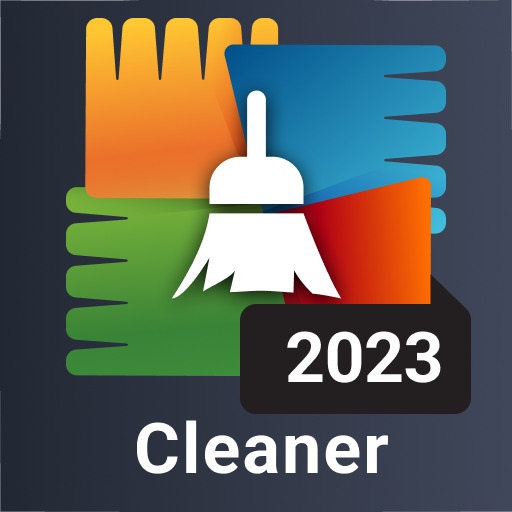
\includegraphics[width=0.4\textwidth]{avg.png}
\end{wrapfigure}

\textbf{1. AVG Cleaner}

\textbf{Developer}: AVG Mobile

\textbf{Description}: AVG is a mobile cleaning tool designed to delete junk files from the phones' storage.

\textbf{Characteristics}:

• \textbf{App analyzer}: The application will identify applications that could be causing mobile data to drain faster;

• \textbf{App remover}: The app can has options for app removal;

• \textbf{Junk cleaner}: The application can delete junk and leftover files;

\textbf{Data security}:

• This application may share data with third parties;

• This application may collect these types of data (Location, Personal info and 3 others);

• Data is encrypted in transit;

• Data can be deleted.\newline

\begin{wrapfigure}{r}{0.4\textwidth} 
    \centering
    
\includegraphics[width=0.4\textwidth]{app2.png}
\end{wrapfigure}

\noindent 
\textbf{2. Phone Cleaner - Cache Clean}

\textbf{Developer}: Games Tree

\textbf{Description}: Phone cleaner is a cleaning app for an Android device and has the following characteristics: file cleaning capabilities, it can cool the CPU, a built-in application manager, and battery-saving functions.

\textbf{Characteristics}:

• \textbf{Cache Cleaner}: The app can clean apps or residual data, such as cache memory;

• \textbf{Storage Cleaner}: This function scans the phone for data to delete and free up space so it can increase the phone's performance;

• \textbf{CPU Cooling}: The app can cool the CPUs temperature and improve its performance;

• \textbf{Battery saving actions}: Another function of the app is the disabling of power-consuming apps;

• \textbf{Notification cleaning functions}: The last function of the app is its notification cleaning capabilities;

\textbf{Data security}:

• No data was collected;

• Data will be encrypted during transit;

• The user can request the data to be deleted;

• No data is shared with third parties.\newline

\begin{wrapfigure}{r}{0.4\textwidth} 
    \centering
    
\includegraphics[width=0.4\textwidth]{app3.png}
\end{wrapfigure}

\noindent 
\textbf{3. CCleaner – Phone Cleaner }

\textbf{Developer}: Piriform

\textbf{Description}: CCleaner helps you remove junk messages from your Android phone. This Android cleaning app clears your browser history, app cache, and clipboard contents. This Android device cleaner also helps to boot faster and provide better performance.

\textbf{Characteristics}:

• The app can clean cache memory, browser memory, and much more;

• Storage cleaning: The app can also analyze storage space and delete unwanted and residual data to boost performance;

• Application hibernation function, which allows the app to keep apps closed until opened manually;

• Ram boosting functions;

• Increases performance and battery life;

• Analyzes the impact of applications;

• Optimizes the storage of photos;

• Monitors the system.

\textbf{Data security}:

• The application may send different types of data to third parties;

• The application may collect the following types of data (Location, Personal Information);

• Data will be encrypted during the transmission period;

• The data can be deleted at request.\newline

\newpage
\begin{wrapfigure}{r}{0.4\textwidth} 
    \centering
    
\includegraphics[width=0.4\textwidth]{1tapcleaner.png}
\end{wrapfigure}

\noindent 
\textbf{4. 1TapCleaner }

\textbf{Developer}: Sam Lu

\textbf{Description}: 1-Tab Cleaner has the ability to clear caches, search histories, and defaults.

\textbf{Characteristics}:

• The app can clean the cache memory;

• Another characteristic is the creation of a list of default apps and the clearing of their selected defaults;

• The application can also clear history data;

• The app can also notify the user if any app uses to much space with its cache memory.

\textbf{Data security}:

• This application doesn't share data with third parties;

• This application may collect these types of data (Location, app info);

• Data is encrypted in transit;

• Data can't be deleted.\newline

\begin{wrapfigure}{r}{0.4\textwidth} 
    \centering
    
\includegraphics[width=0.4\textwidth]{app6.png}
\end{wrapfigure}

\noindent 
\textbf{5. Droid Optimizer }

\textbf{Developer}: Ashampoo®

\textbf{Description}: Droid Optimizer is an application that aims to monitor the phone's battery, notify the user of the remaining battery time, optimize the phone and automatically perform cleaning tasks.

\textbf{Characteristics}:

• The application can perform cleaning tasks automatically;

• The application can also find and delete unwanted files;

• Clears system and application cache;

• The application employs different methods for saving energy and improving battery life;

• The application can disable WI-FI at predetermined times or every time the screen is turned off;

• Manages applications;

• The app has the option to expose apps that spy on their user and that have critical permissions.

\textbf{Data security}:

• No data is shared with third parties;

• This application may collect these types of data: Location, application activity, and application information and performance;

• Data is encrypted in transit;

• Data cannot be deleted.

\newpage


\section{Comparison}\label{sect:comparison}
    Each application presented has some specific characteristics, and although most of them have similar features, each one brings something different:

    1.	Droid Optimizer automatically turns off the user's mobile data and lets the user take a look at critical app permissions, exposing spy apps;
    
    2.	1TapCleaner allows the user to delete search histories and defaults and can notify the user if any app uses too much space for its cache memory;

    3.	CCleaner optimizes photo storage and presents the Task Killer functionality;

    4.	Phone Cleaner presents the Notification Cleaner functionality that deactivates and deletes unwanted notifications, if necessary;

    5.	AVG Cleaner has the ability to clean applications that drain mobile data.

    One drawback of these applications is the frequent use of free trials, ads, and such that either ruin the user experience or lock the user behind a paywall.
    
    From the point of view of data security, Droid Optimizer, 1TapCleaner, and Phone Cleaner do not share data with third parties while CCleaner and AVG Cleaner share data, and from the point of view of data collection, Battery Guru and Phone Cleaner do not collect, while the rest of the applications collect data. 

    For the purpose of creating an application that offers a similar function as the ones listed above, the app should not be a one-to-one copy of another, as such, we need to look at these sorts of comparisons, to better understand what could be improved upon and added. For example, the proposed app of this paper looks at different types of files to delete, checks up on apps by their last time being used, and checks the trash folder for potential residual files. In the following page, we will look at a comparison table that looks at what each application offers, providing a clear view of each functionality listed above and which app either has such an option or not.

    \begin{center}
    \begin{tabular}{ | >{\centering\arraybackslash}X m{3cm} | >{\centering\arraybackslash}X m{1.8cm} | >{\centering\arraybackslash}X m{1.8cm} | >{\centering\arraybackslash}X m{1.8cm} | >{\centering\arraybackslash}X m{2.2cm} | >{\centering\arraybackslash}X m{2cm} | }
    \hline
        \textbf{Comparison} & \textbf{AVG Cleaner} & \textbf{Phone cleaner} & \textbf{CCleaner} & \textbf{1TapCleaner} & \textbf{Droid Optimizer} \\ \hline

        Cache cleaning options & NO & YES & YES & YES & YES \\ \hline

        Disable WI-FI & NO & NO & NO & NO & YES \\ \hline

        Notify the user if any app has cache memory that consumes too much memory & NO & NO & NO & YES & NO \\ \hline

        Analyze application impact & YES & NO & YES & NO & NO \\ \hline
        
        RAM Boosting options & NO & NO & YES & NO & NO \\ \hline

        System monitoring & NO & NO & YES & NO & NO \\ \hline

        Clear Defaults options & NO & NO & NO & YES & NO \\ \hline

        Clear history options & NO & YES & NO & YES & NO \\ \hline

        CPU cooling options & NO & YES & NO & NO & NO \\ \hline
        
        Application Manager & NO & NO & NO & NO & YES \\ \hline
        
        Managing critical permissions & NO & NO & NO & NO & YES \\ \hline
        
        Data collection & YES & NO & YES & NO & YES \\ \hline
        
        Optimizing the storage of photos & NO & NO & YES & NO & NO \\ \hline
        
        Memory space recovery & YES & YES & YES & YES & YES \\ \hline
        
        Notification cleaner & NO & YES & NO & NO & NO \\ \hline
        
        Sharing with third parties & YES & NO & YES & NO & NO \\ \hline
        
        Encrypted data in transit & YES & YES & YES & YES & YES \\ \hline
        
        Data may be deleted & NO & YES & YES & NO & NO \\ \hline
        
    \end{tabular}
\end{center}

%%%%%%%%%%%%%%%%%%%%%%%%%%%%%%%%%%%%%%%%%%%%%%%%%
%%%%%%%%%%%% chap: App Arhitecture %%%%%%%%%%%%%%%%%
%%%%%%%%%%%%%%%%%%%%%%%%%%%%%%%%%%%%%%%%%%%%%%%%%

\chapter{App Arhitecture }\label{chapter:chap2}

\section{Use Cases Diagram and Sequence Diagram}\label{sect:initial use cases diagram}

\begin{figure}[htp]
    \centering
    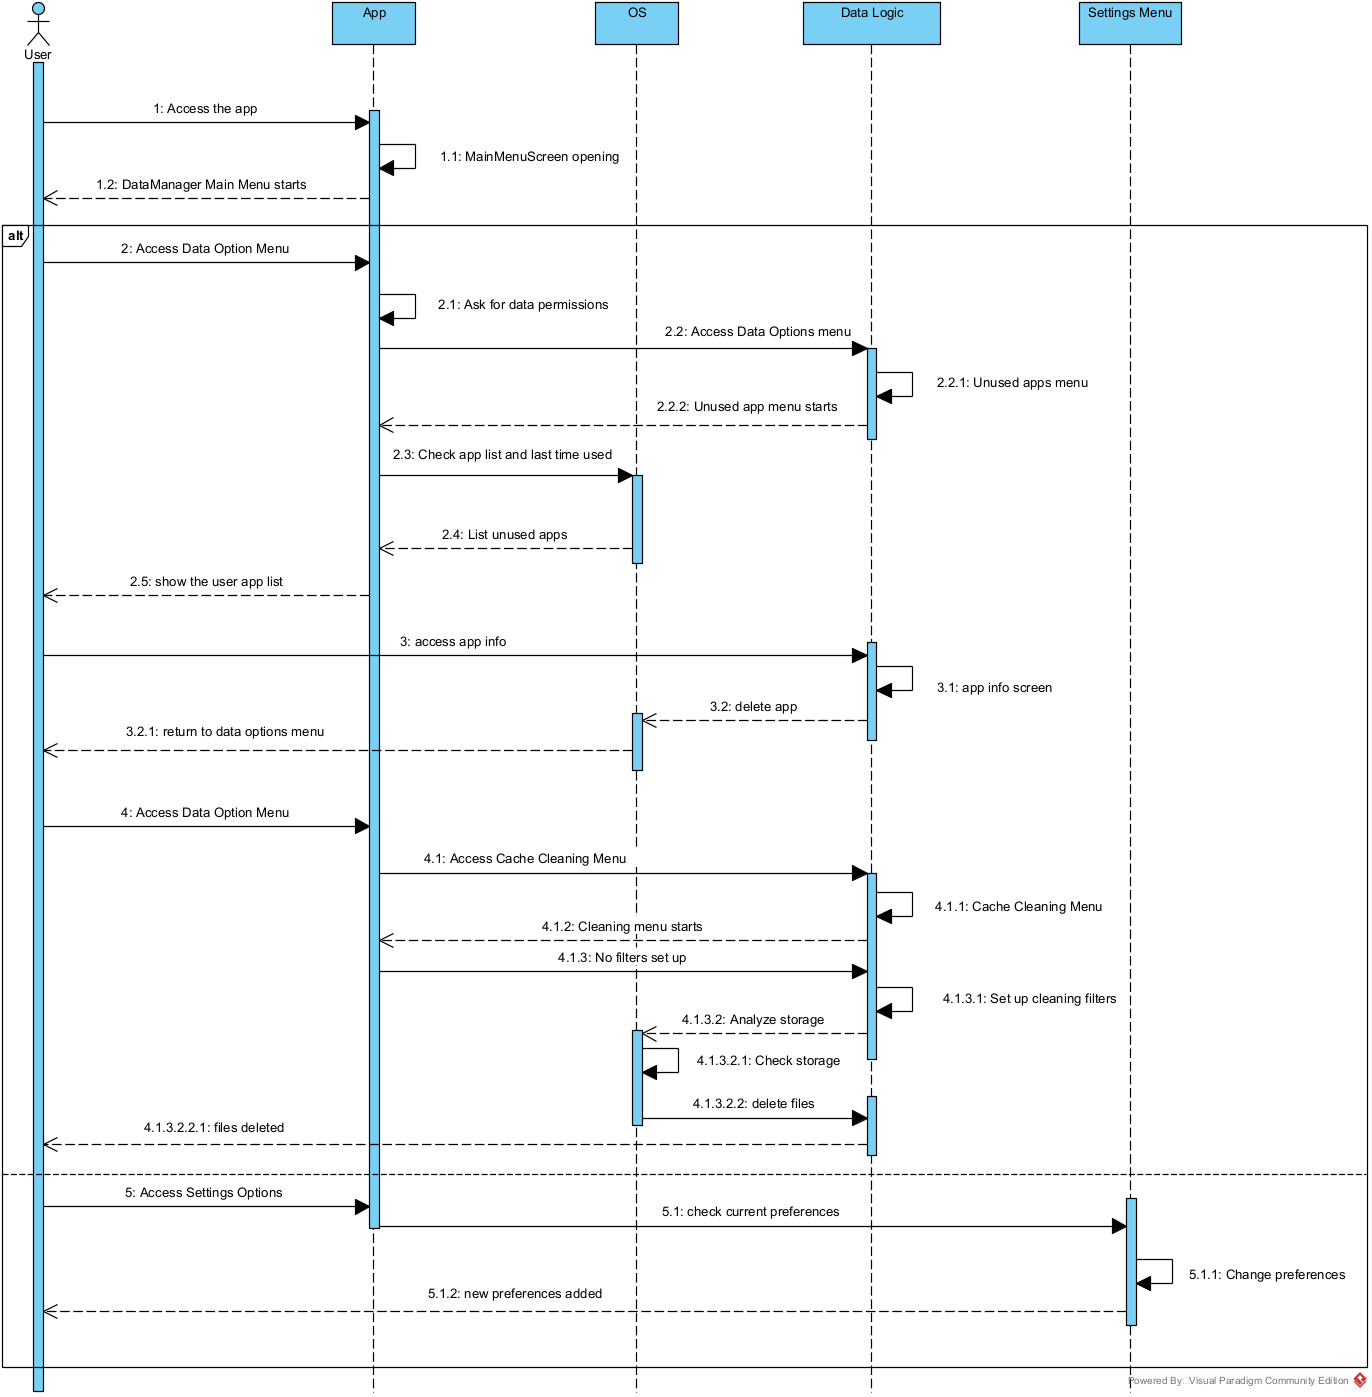
\includegraphics[width=340pt]{Basic Flow2.png}
    \caption{Basic Flow}
    \label{fig: Sequence Diagram}
\end{figure}

The main flow that the application will follow. It starts with the main menu screen, where the user can either access the data option menu or the settings menu. 

The 2 screens have the following functionalities: the settings menu will offer the option to change the theme of the application, change the language of the text inside the application, and read, in a new menu, some information about it, while the data options menu has the cache cleaning scree, where the user can delete unneeded files by setting up filters for them, and the unused applications list, where the user can find what applications he doesn't usually use.

The diagram has one actor, the user, and 4 lifelines, the \ac{OS}, data options menu, settings menu, and the app itself.

\begin{figure}[htp]
    \centering
    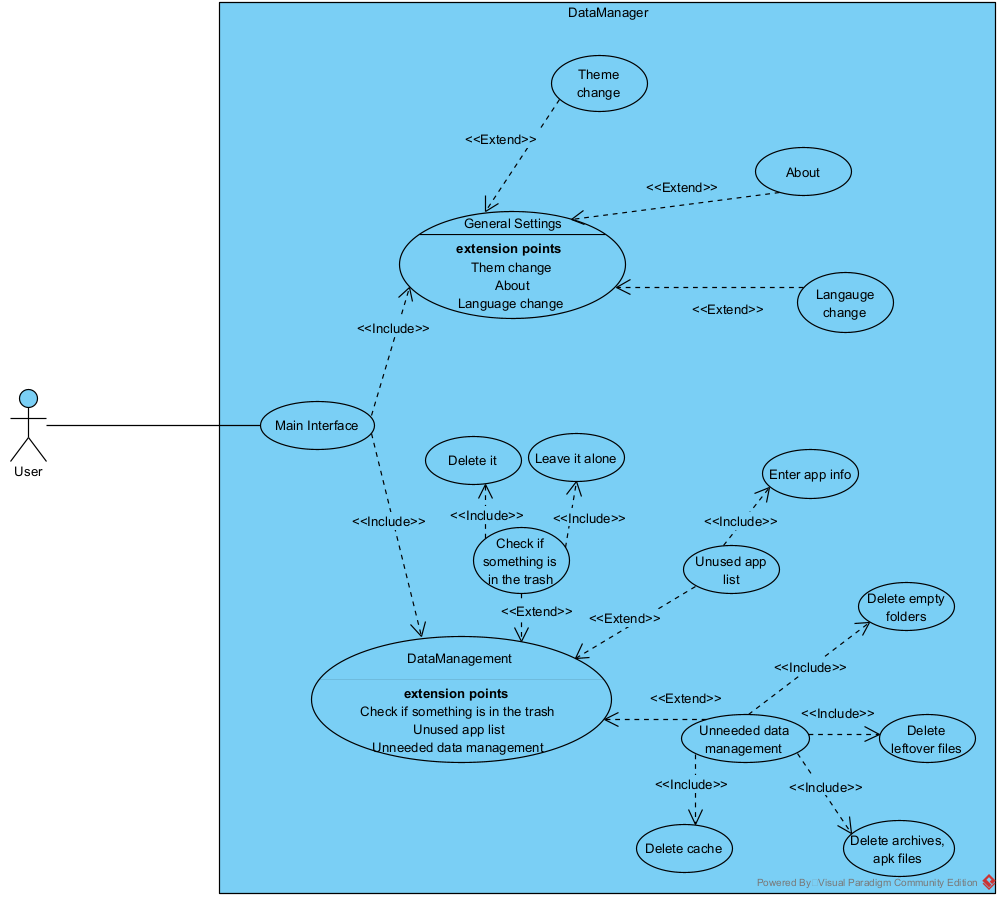
\includegraphics[width=360pt]{UseCases2.png}
    \caption{Use Cases Diagram}
    \label{fig: Use Cases}
\end{figure}

The above diagram shows the use cases of the application, what the user has access to, and the decision he can make with the options provided.
    
    The 3 main functionalities that the app offers are as follows:

    • The option to delete \ac{APK} files, cache files, archived files, leftover files, and empty folders from the storage of the phone, each type of file having a filter slider that can be turned on or off;

    • Check whether or not there are files in the trash can and the option for the automatic deletion of what's in it;

    • A general setting area where the user can change the theme and language of the app, while also being able to access an about menu for information about the application;

    • The application also has a percentage estimate for the remaining battery life and remaining storage space
    
\newpage


\newpage

\section{App Architecture}\label{sect:app architecture}

\begin{figure}[htp]
    \centering
    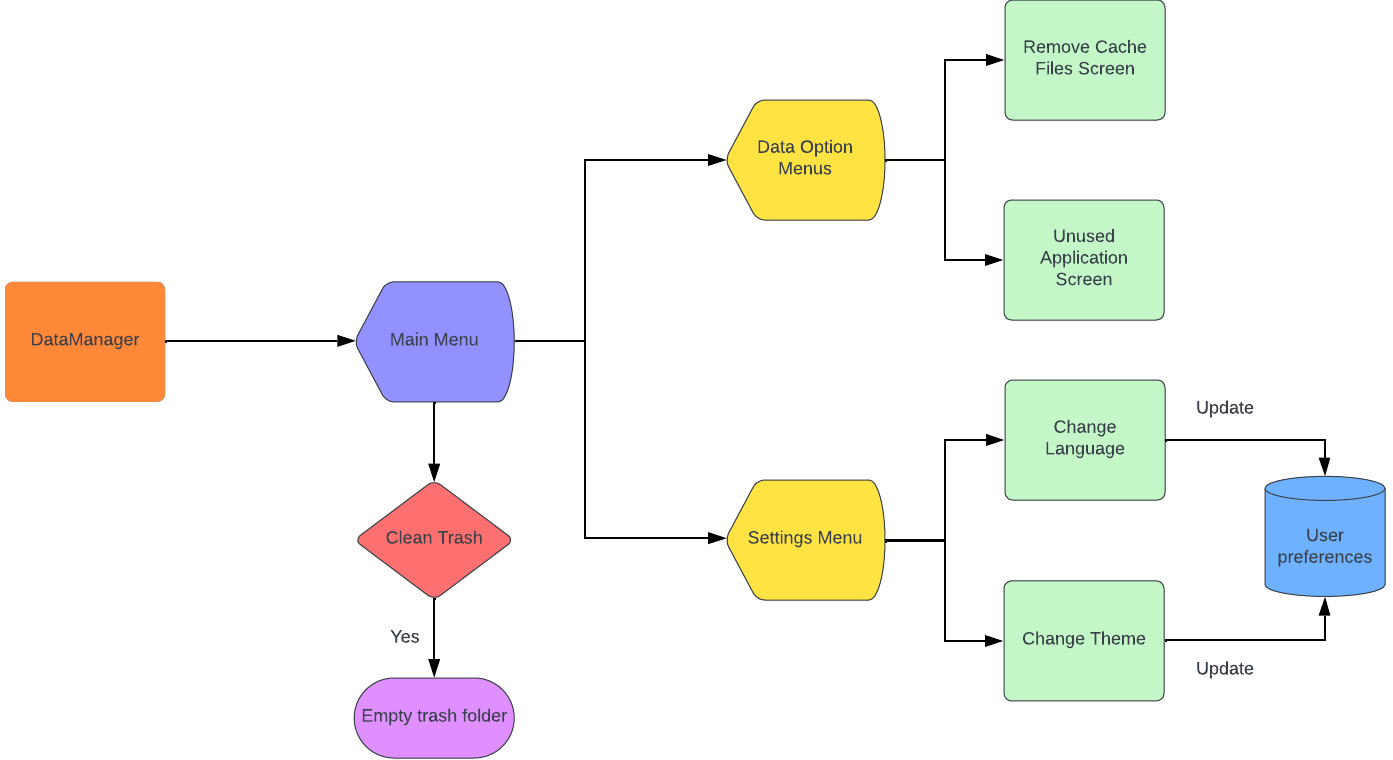
\includegraphics[width=450pt]{App_Arhitecture2.png}
    \caption{App Arhitecture}
    \label{fig: App Arhitecture}
\end{figure}

This figure presents how the app will function, when it starts, it will display a general \ac{UI} interface where the user can go between the data options and settings menu. The data options menus can delete unneeded data and scan the phone for a list of all applications and the last time they were used. 

The other functionalities that the app offers, are the settings menu where the user can set up a different or a different language, and look at an about menu to learn more about the app. These preferences will be saved in a database for the convenience of the user so as to not set them each time they exit and enter back on the application. 

The last functionality is the one for emptying the trash folder, a function that when clicked, the user will be alerted if he still wants to go through with this option or not.

Chapter 5 will delve deeper into each screen and how should it be used, while Chapter 4 will focus on the implementation of the application.

%%%%%%%%%%%%%%%%%%%%%%%%%%%%%%%%%%%%%%%%%%%%%%%%%
%%%%%%%%%%%% chap: Implementation \& Results%%%%%%%%%%%%%%%%%
%%%%%%%%%%%%%%%%%%%%%%%%%%%%%%%%%%%%%%%%%%%%%%%%%

\chapter{Implementation Logic}\label{chapter:chap4}

\section{System Requirments \& Technologies Used}\label{sect:System Requirments \& Technologies Used}

For the implementation of the proposed app, the development medium chosen was Android Studio, while the programming language used was Kotlin. Details on all technologies used are as follows:\\

\textbf{\ac{IDE} used: }  \\
Android Studio \cite{1} is an official \ac{IDE} for Android app development, based on the tools offered by the IntelliJ IDEA, which is designed with powerful features for increased productivity in app development. The features on offer by Android Studio are as follows: a Gradle-based build system, an emulator for testing and experimenting on the apps developed, offering for the user the ability to test his or her application on different \ac{API} levels, and personalize their emulator settings for varied testing environments, the ability to develop applications for all Android devices, the ability to edit and update composables in real-time while the emulator or physical device is running. The \ac{IDE} also offers different code templates, testing tools, and frameworks for an increase in productivity and development time, while also including a GitHub integration and support for C++ and \ac{NDK}.
\\

\textbf{Programming Language used: } \\
Kotlin \cite{5} is a cross-platform, general-purpose programming language developed and released in 2011 by JetBrains, being built as a statically typed language, meaning that the variable type is going to be known at compile time. One key feature of Kotlin is in its design policy, the language being developed to be fully interoperable with Java, making the use of Java and Kotlin, in the same project, possible. With it being a concise, and safe programming language, it is usually recommended the use of Kotlin in applications development, being more often than not the best choice for such projects. The main reasons why Kotlin is a good choice for development stems from its many features that allow its users to write code in an easier manner, such as null safety, coroutines used for asynchronous programming, and extension functions. 

\newpage

\textbf{Database technology used: } \\

Firebase \cite{2} is an app development platform that offers a variety of tools and services to help in the development of high-quality applications. 

One of the key features of Firebase is the Firebase Realtime Database \cite{3}, which is a cloud-hosted database. The data is stored in a \ac{JSON} file, letting the user store and sync data in real-time, for every connected client. Such features help when building cross-platform applications, with all clients sharing one Realtime Database instance and automatically receiving updates with the newest data.

\textbf{Other technology used: } \\

Other technologies used include the Jetpack Compose toolkit, used for the UI layout, and the use of XML files which were used for certain screen layouts, strings, color pallets, permission, component definition, various graphical elements, and so on.

Jetpack Compose \cite{4} is a toolkit designed for building Android \ac{UI}. Its main benefits consist of simplifying and accelerating \ac{UI} development on Android by allowing by providing the user with a set of powerful tools, and intuitive Kotlin \ac{API}s, being fully declarative, which means that the \ac{UI} elements can just be described and Compose will take care of the rest. Another big benefit of Compose is that the \ac{UI} automatically updates.

XML files are used in Android Studio and app development for several purposes, such as:\\
    • Layout: This type of XML file is used to define the general layout of the user interface, holding all elements such as text views, buttons, sliders, and others;\\
    • Strings: This file is used as an alternative for hard-coded strings. They define strings that can be accessed throughout the entire app, being especially useful for changing the text of an app from one language to another;\\
    • Colors: This XML file is used to define different colors that the user can use throughout the application, this file is especially useful when changing the theme of an app;\\
    • Drawables: These are XML files that are used to create various graphic icons or images;
    • Manifest: Lastly, these files are used to define the components of the application, including the packages, activities, receivers, and permissions that the application needs;\\
\\
For testing, the app was experimented on the emulators provided by Android Studio, on an emulator with \ac{API} 30 and 33, and the app was also tested on different physical devices, mainly a Samsung J6, and a Samsung A 54.

The basic system requirements for running the app are as follows:

    • An Android phone with the Android Version 11+;
    
    • Connection to the Internet;
\newpage
\section{Implementation}\label{sect:Implementation}

\subsection{Main Menu Implementation}\label{subsect:Main Menu Implementation}

\begin{figure}[htp]
    \centering
    \begin{minipage}{0.45\textwidth}
        \centering
        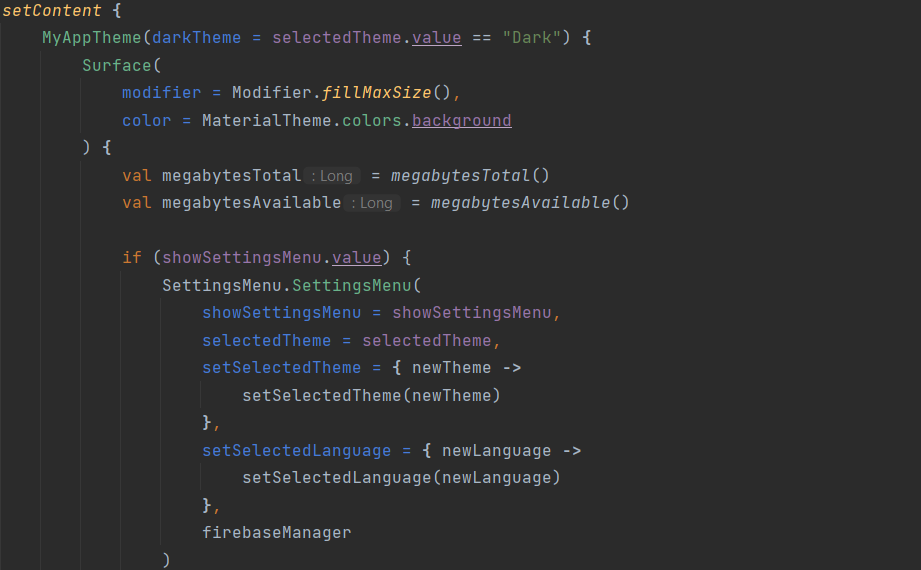
\includegraphics[height=240pt, width=260pt]{setContent1.png}
    \end{minipage}\hfill
    \begin{minipage}{0.45\textwidth}
        \centering
        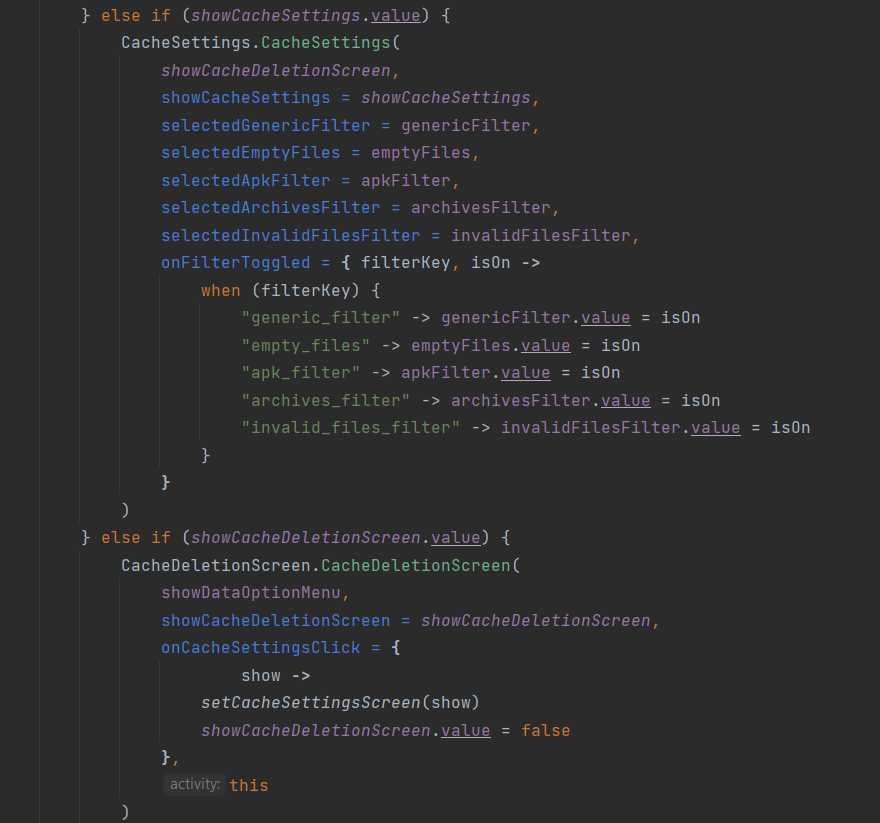
\includegraphics[width=260pt]{setContent2.png}
    \end{minipage}
    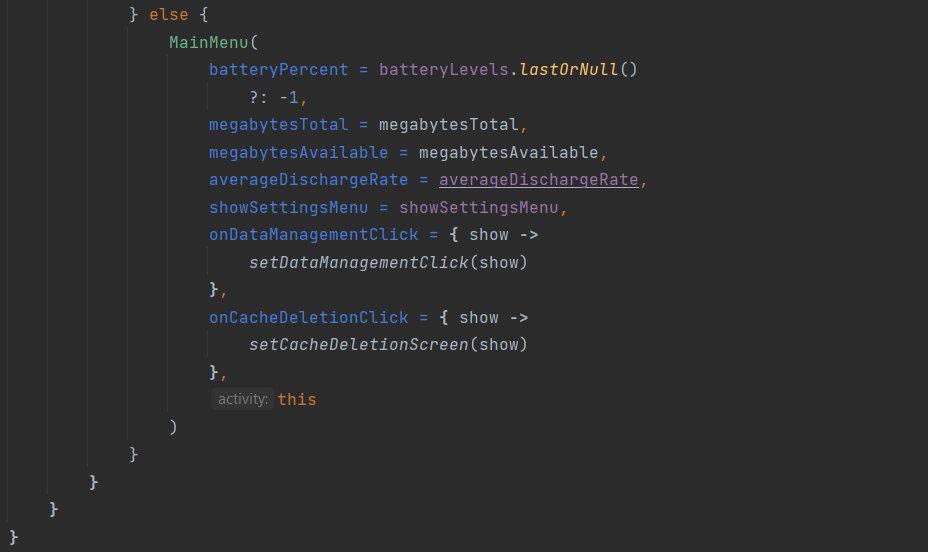
\includegraphics[width=260pt]{setContent3.png}
    \caption{Set Content}
    \label{fig: SetContent}
\end{figure}

Figure 4.1 shows the logic behind screen hopping, the app is actually composed of only two activities, the main activity and the permission activity, the content of the main activity being created through the setContent() method.

As such, the main activity sets up screens and values for whether these screens are shown or not. The main screen is the main menu, where the user accesses the other screens. Each screen is built with a composable, with the bulk of the \ac{UI} elements being comprised of Material3 elements.



\newpage
\begin{figure}[htp]
    \centering
    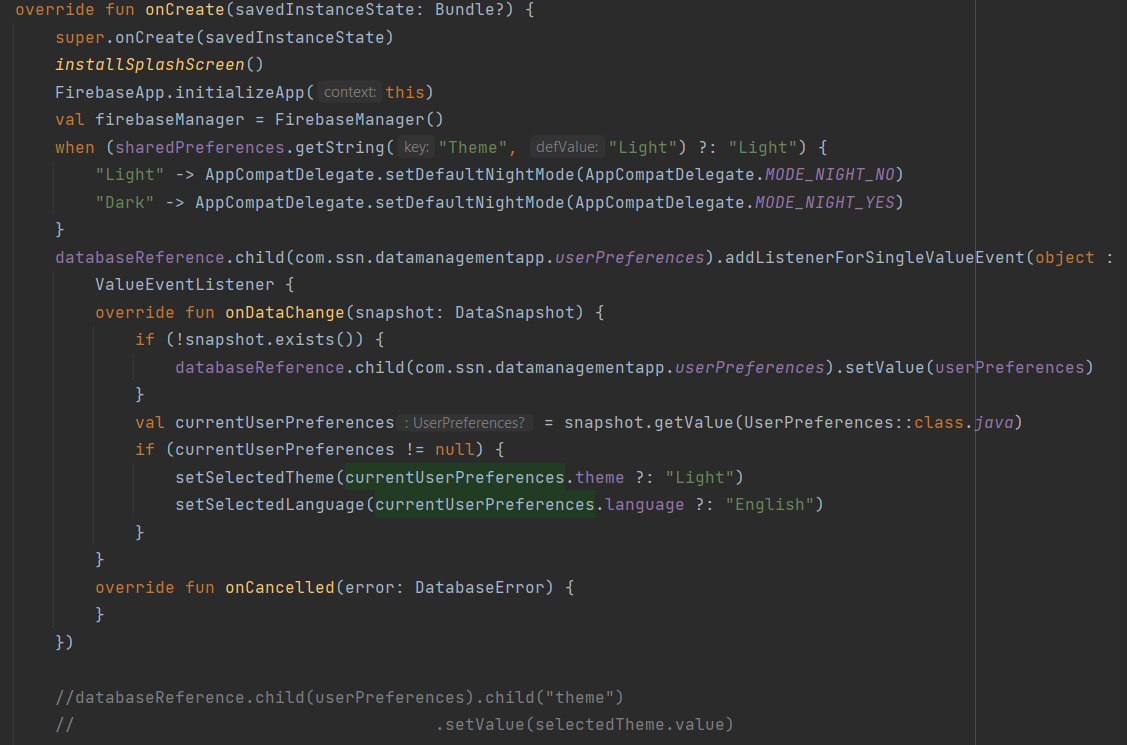
\includegraphics[width=380pt]{Firebase1.png}
    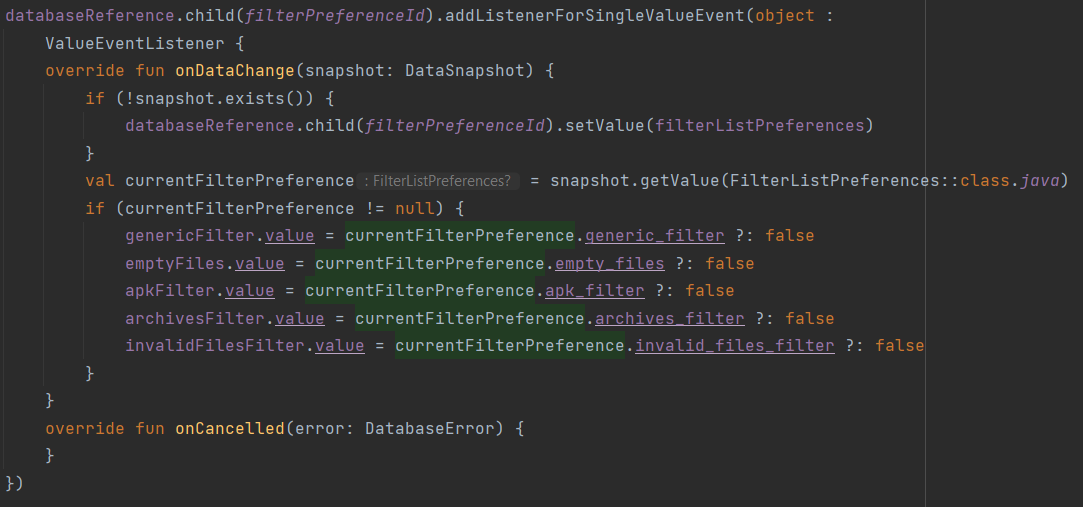
\includegraphics[width=380pt]{Firebase2.png}
    \caption{Firebase fetch \& update data}
    \label{fig: Firebase fetch & update data}
\end{figure}

In the above figure, 4.2, the onCreate function is called, which is a function usually called when first entering the application. It is here the basic logic of the application takes place, like the Firebase setup and preference assignation.

After which, we can see how the FirebaseApp is initialized, how the app selects the theme when the application is started, and how the data for the user preferences is being assigned at the beginning of the app, the values being assigned from the databaseReference value. At the beginning of the onDataChange method, if the collection userPreferences doesn't exist, if so, the app creates it. Then, the app assigns the current value for each preference value and updates the \ac{UI} accordingly.

Below it, the same operation is taking place for the preferences set by the user for the file filters that will be used for the cache deletion screen.
\newpage

\begin{figure}[htp]
    \centering
    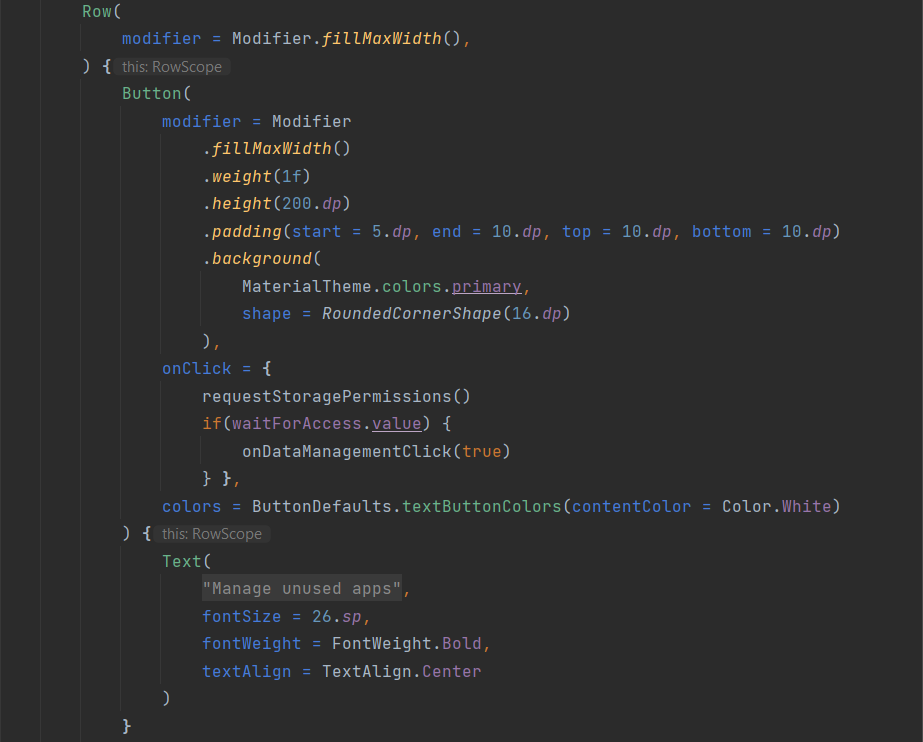
\includegraphics[width=460pt]{buttonexample.png}
    \caption{Button Implementation Example}
    \label{fig: Button Implementation Example}
\end{figure}

Here, figure 4.3, shows an example of the implementation of a button for menu hopping between the screens of the application. Most buttons throughout the app have a similar structure, utilizing Material3 elements, and the logic set up in the Main Activity for going through different menus.

For better alignment, a row composable is added, with a modifier to fill the maximum width of the screen. The button is then created, utilizing a button compose of the following variables: modifier, which is used for the shape of the button and the background color of it, onClick, which is used for managing the action that takes place when the button is clicked, and colors, which is used to color the text composable inside the button. The text composable has set up custom text alignment, custom font size, and weight, and for the text itself, the app uses the following method: context.getString(R.string.textdatamanagement), context is used as an instance for the current activity that is running, while R.string is used by the app to communicate with the file strings.xml, which holds various strings for ease of use and ease of potentially changing the application's language.

\newpage

\subsection{Settings Menu Implementation}\label{subsect:Settings Menu Implementation}

\begin{figure}[htp]
    \centering
    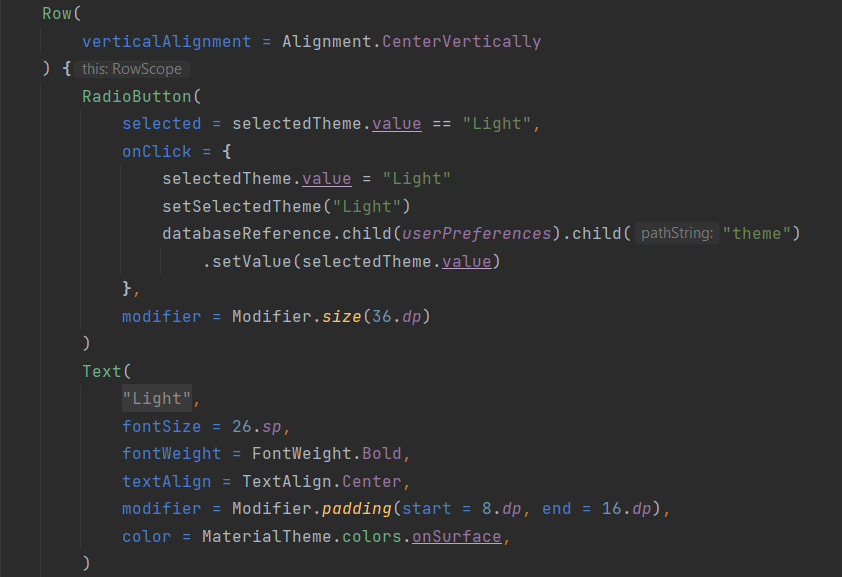
\includegraphics[width=380pt]{light.png}
    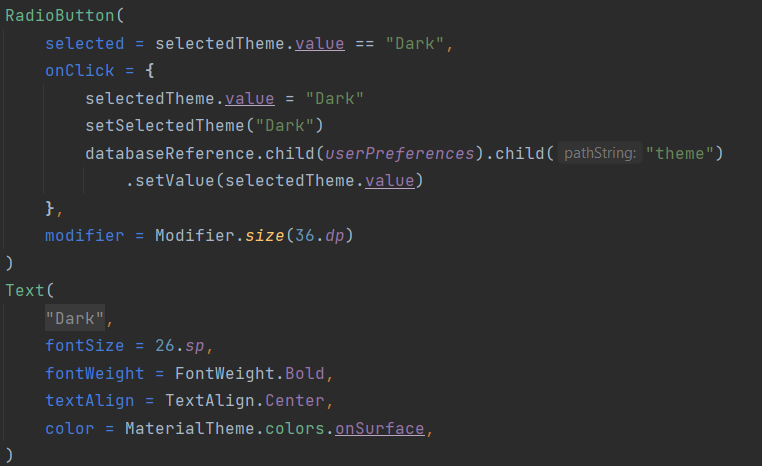
\includegraphics[width=380pt]{dark.png}
    \caption{Theme Options}
    \label{fig: Theme Options}
\end{figure}

Figure 4.4 showcases the implementation of theme options. For that, a set of radio buttons was preferred, the first radio button being used for the light theme, while the second being used for the dark theme. After clicking on one of the radio buttons, the other button is closed, and the changes are updated as well in the Firebase Database, where the theme value is updated accordingly.

SelectedTheme is used as a way to check which radio button should be checked, while setSelectedTheme is used to set for the whole app the new theme is chosen.

As mentioned in the explanation of Figure 4.3, the way these elements are created consists of composable functions, each having the benefit of being easy to use.

\newpage

\begin{figure}[htp]
    \centering
    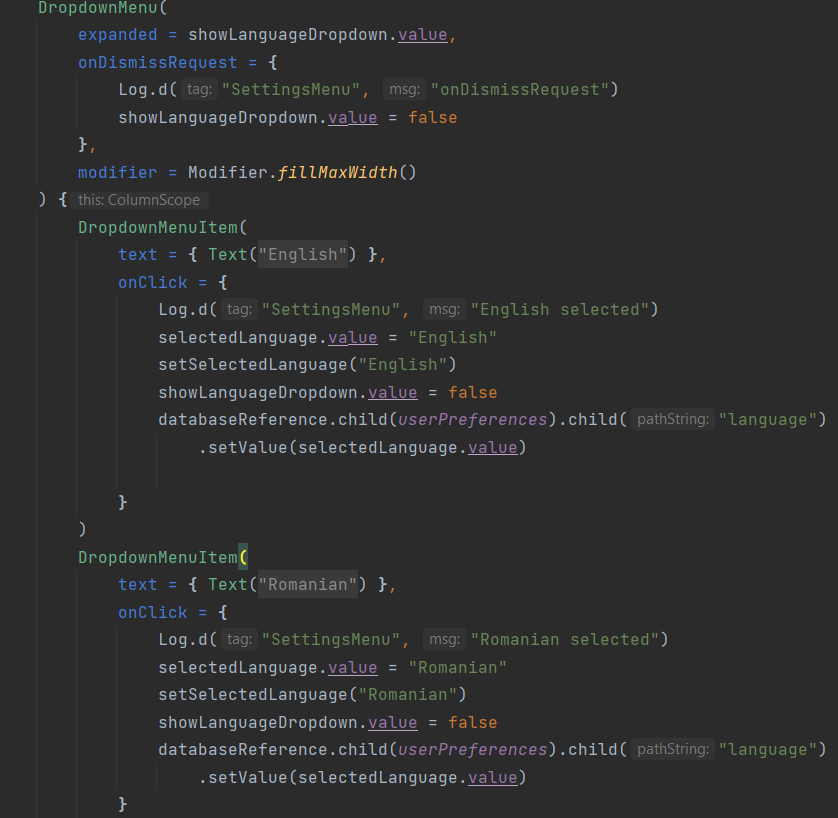
\includegraphics[width=450pt]{language.png}
    \caption{Language Dropdown Menu}
    \label{fig: Language Dropdown Menu}
\end{figure}

Here, in Figure 4.5 can be seen the implementation for the language dropdown menu, where the user can choose either Romanian or English as the preferred language for the application.

A DropdownMenu composable was used to achieve this, the menu showing up only when the user clicks on an icon with a text called Language, and closing after the user chooses a language. The menu is populated by items made with the composable DropdownMenuItem which hold text and a clickable button that selects the new language and calls a function inside the main activity that changes the text to the desired language.

\newpage

\begin{figure}[htp]
    \centering
    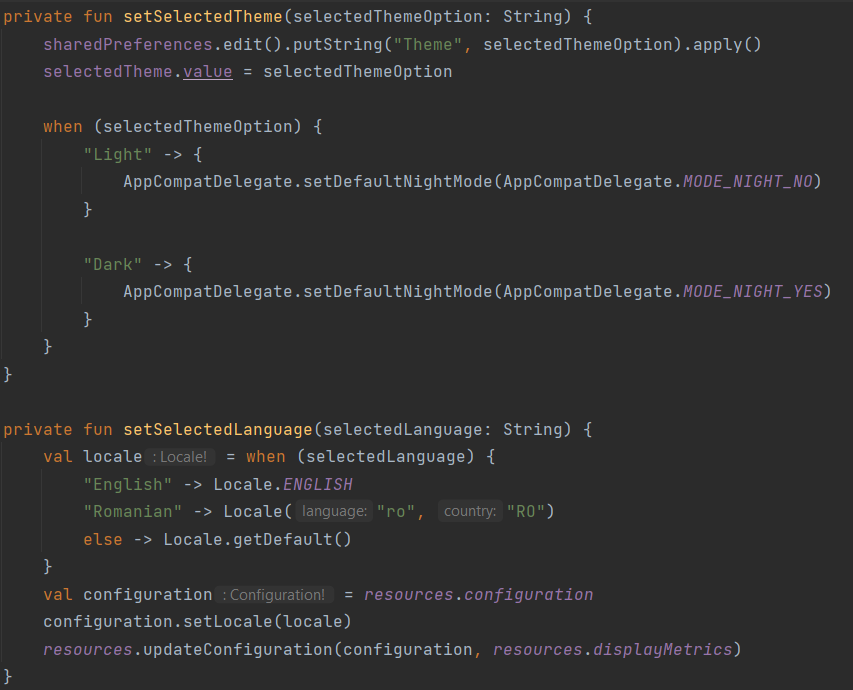
\includegraphics[width=460pt]{setPreferences.png}
    \caption{Theme Options}
    \label{fig: Applying the preferences}
\end{figure}

Figure 4.6 showcases how the language and theme are being applied, the code being found in the main activity class.

For the theme, the main activity looks at the sharedPreferences and edits them by applying the new selected theme. If the theme is selected as light, the app turns off night mode, while if the theme selected is the dark one, the night mode is turned on.

The language is applied by selecting the Locale as either English or Romanian, this object is used to define what language, symbols, and so on should be used.

\newpage

\subsection{Cache Deletion Screen Implementation}\label{subsect:Cache Deletion Screen Implementation}

\begin{figure}[htp]
    \centering
    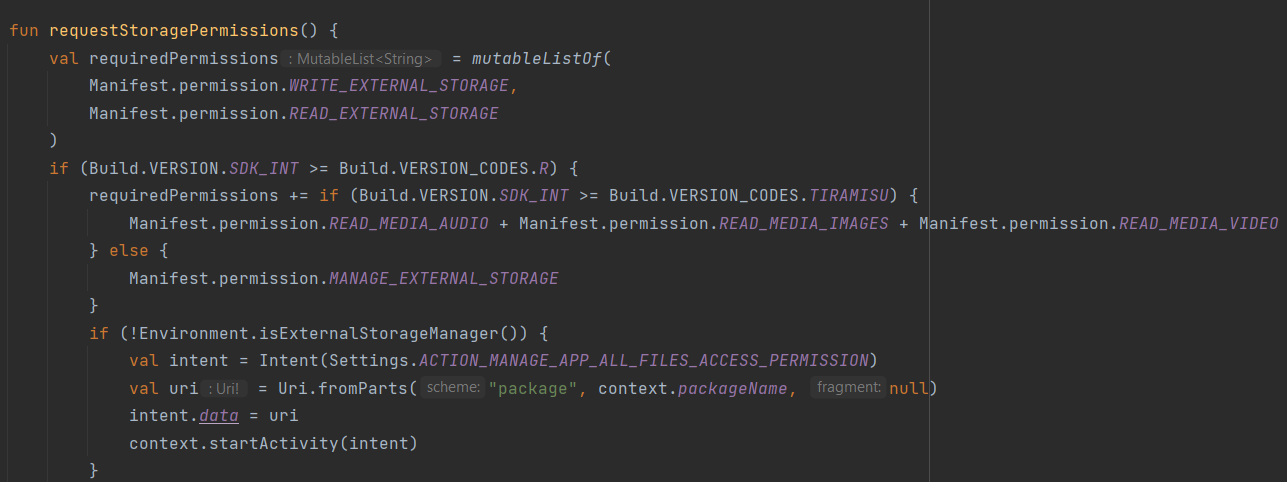
\includegraphics[width=400pt]{permission1.png}
    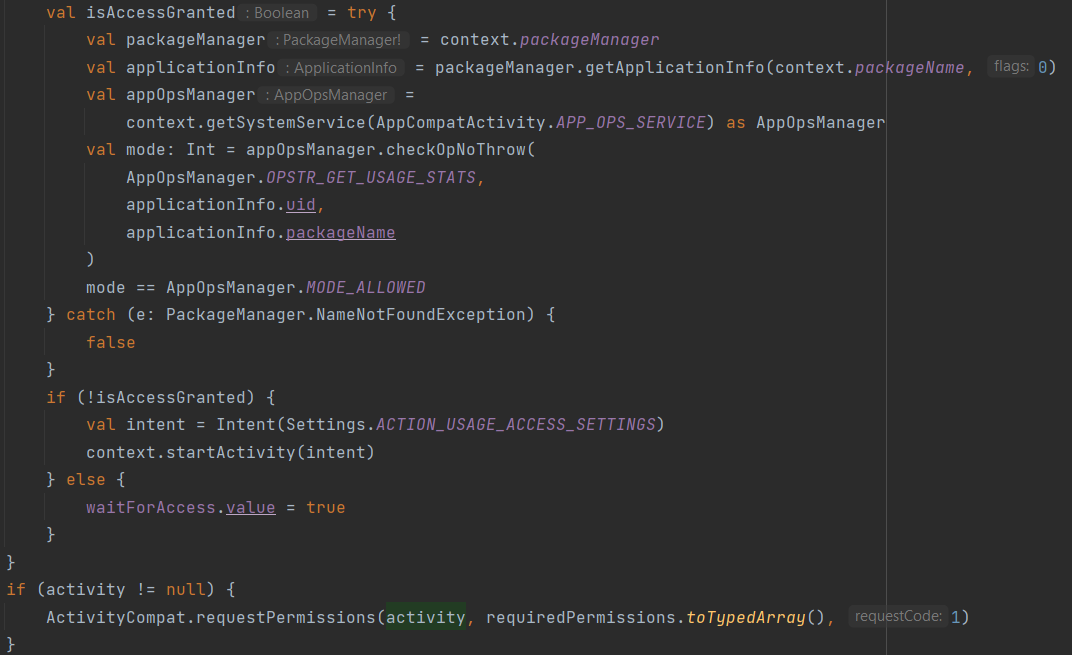
\includegraphics[width=400pt]{permission2.png}
    \caption{Permission Activity}
    \label{fig: Permission Activity}
\end{figure}

Firstly, the application requires some permissions from the user. As such, the above figure shows the logic for asking for such permissions. Firstly, it checks the Android version and adds the required permissions to a list. It then checks if the usage access is granted and starts an activity to request permission if it is not granted. Lastly, the function uses ActivityCompat.requestPermissions to request storage permissions from the user.

\newpage

\begin{figure}[htp]
    \centering
    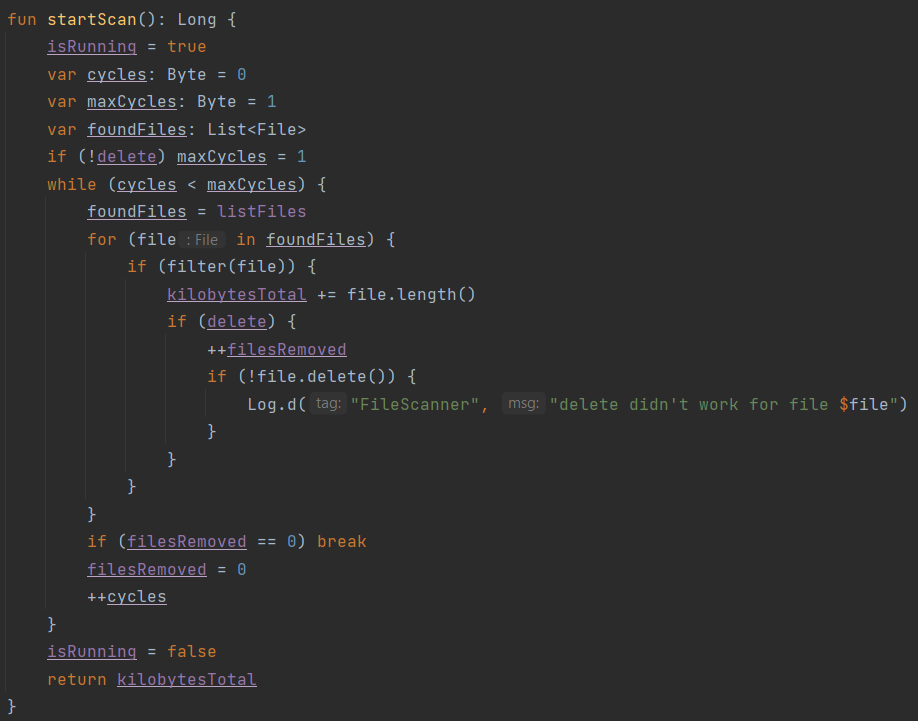
\includegraphics[width=290pt]{cache 1.png}
    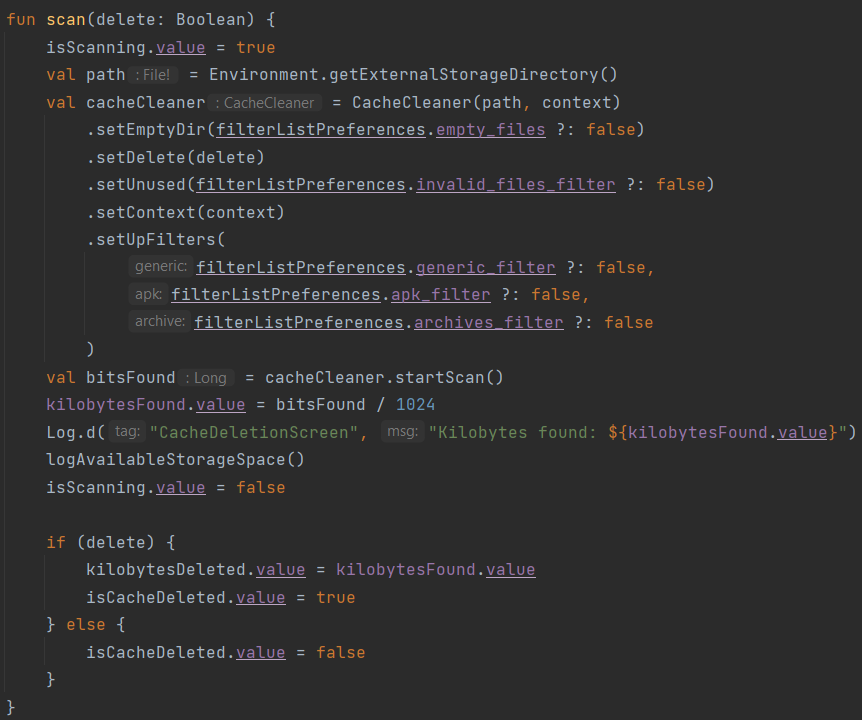
\includegraphics[width=290pt]{cache 2.png}
    \caption{File Scanner}
    \label{fig: File Scanner}
\end{figure}

The Cache Screen consists of two main buttons, analyze and delete. Both of these buttons are created using compose functions like text, buttons, and so on. However, the main point of this app is the scanning feature. As such, when the user presses one of the buttons, the app utilizes the function defined in Figure 4.8. 

Scan() gets the general path of the external storage and creates an instance of the CacheCleaner class that sets up various filters for the type of files the user wants to delete and passes a value for delete, whether the user wants to remove or not the files scanned. To compute the number of kilobytes found, the method uses the CacheCleaner instance to start another function for the proper scanning.

The function startScan() first creates a list of all the files in the storage and then begins going through each one and selecting only those that have their respective filter set on. If the delete value is set to true the removing process can begin and all selected files are deleted from the system. Finally, the app returns the amount of memory it has freed up.
\newpage

\subsection{Unused App Screen Implementation}\label{subsect:Unused App Screen Implementation}


\begin{figure}[htp]
    \centering
    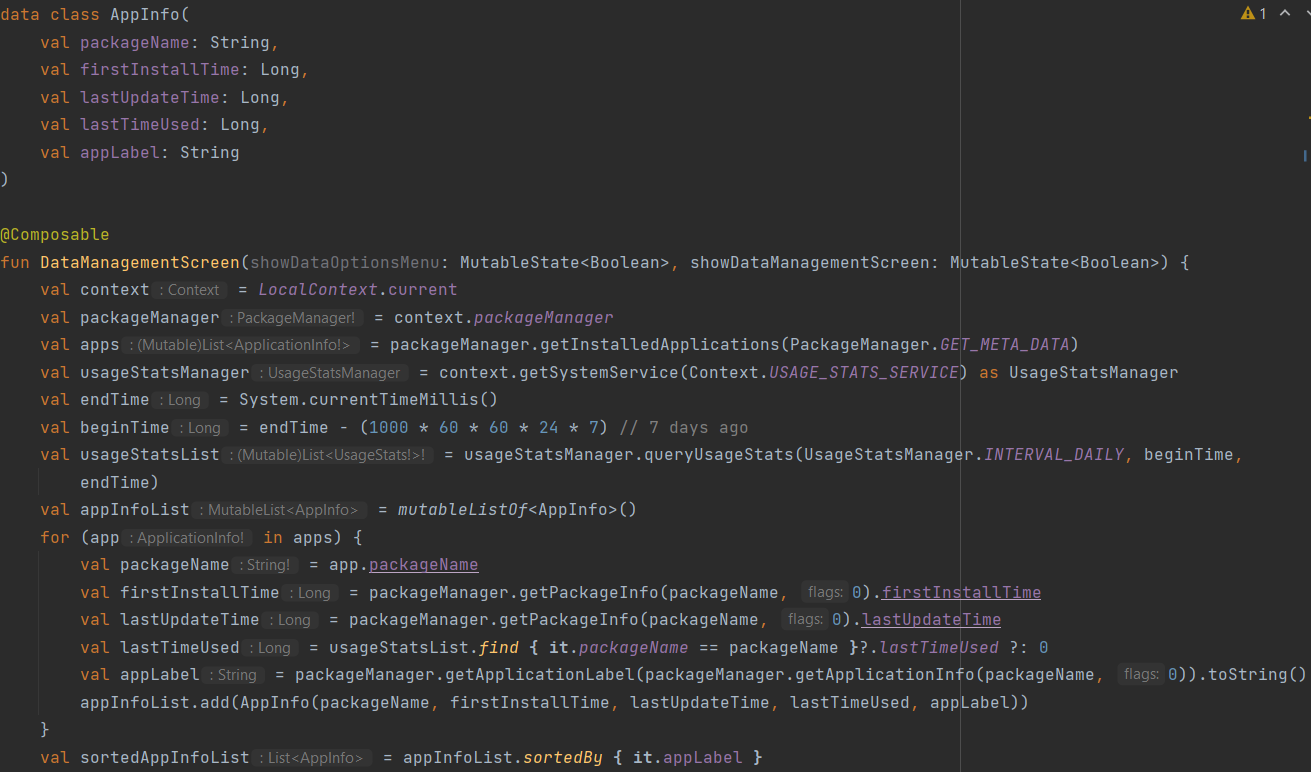
\includegraphics[width=340pt]{unused.png}
    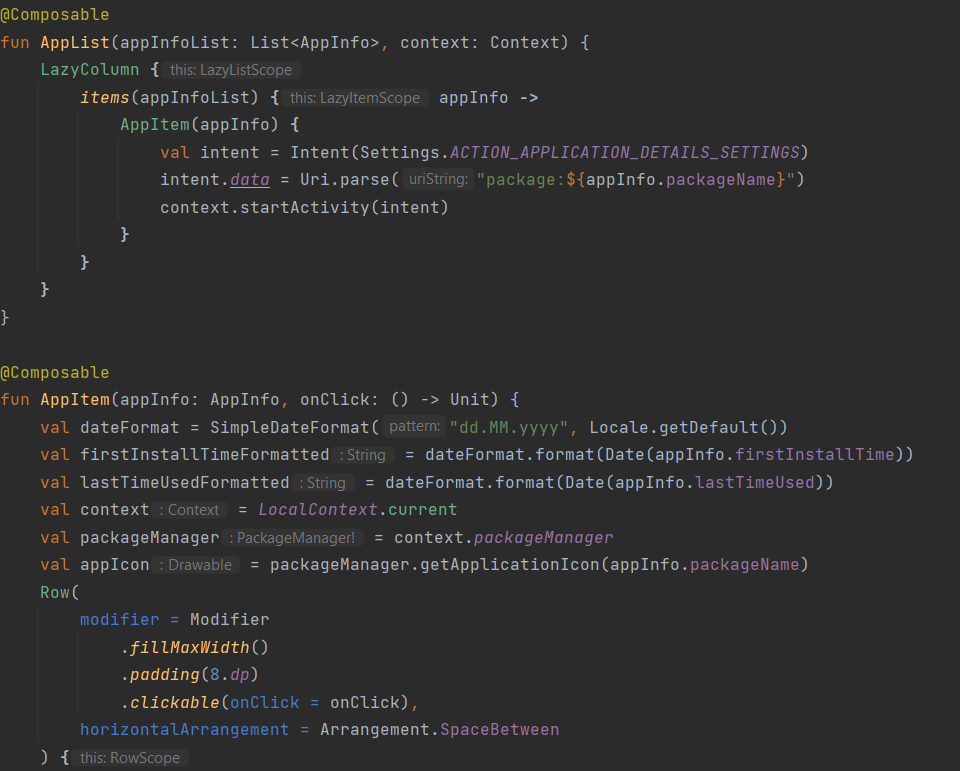
\includegraphics[width=340pt]{unused2.png}
    \caption{File Scanner}
    \label{fig: File Scanner}
\end{figure}

The following Figure, 4.9, shows the logic behind the unused app list. The app list is given through a package manager which retrieves all applications which are then sorted by alphabetical order. The usage stats manager retrieves all the information on when the application was used, when was it installed and when was it last updated.

The composable function AppList assigns to each app their respective app info screen so that when one of the applications in the list is clicked, the app info activity and screen are opened.

AppItem is used to create the visual representation for each application in the list.

\newpage

\subsection{Trash Emptying Implementation}\label{subsect:Trash Emptying Implementation}

\begin{figure}[htp]
    \centering
    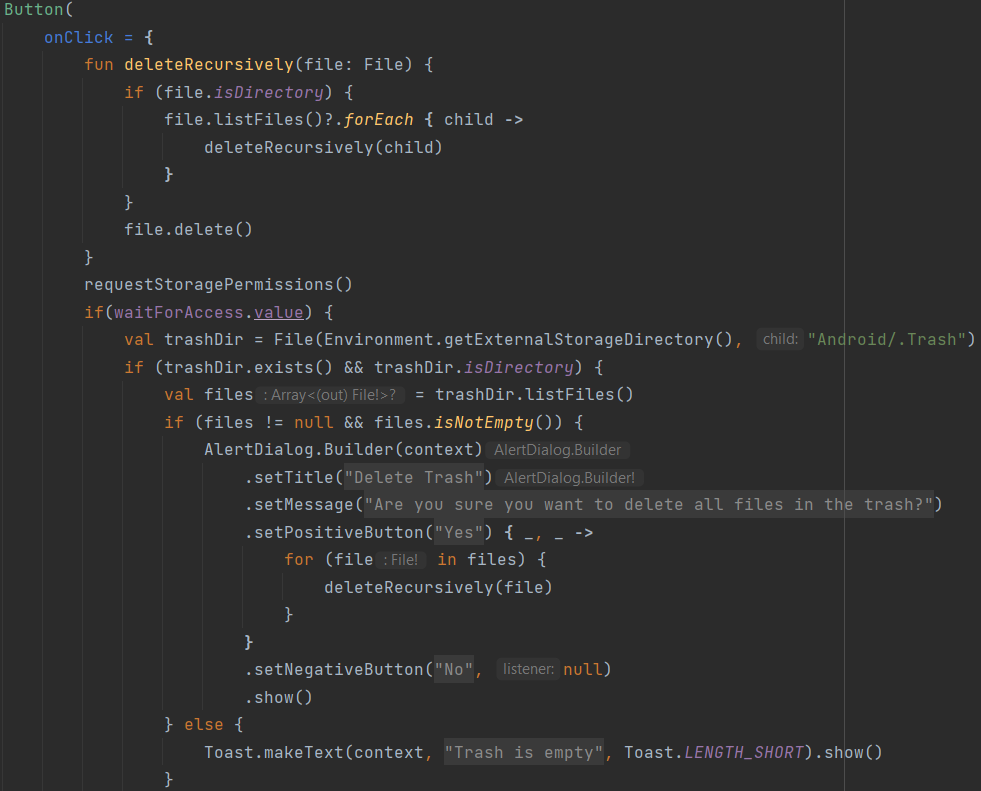
\includegraphics[width=450pt]{trash1.png}
    \caption{App Info}
    \label{fig: Emptying trash logic}
\end{figure}

The last Figure, 4.10, shows the logic for emptying the trash folder, it first requires the needed permissions, and if they are granted, the app will check for the existence of the trash directory. If it exists, the app lists the files inside it and starts recursively deleting them after creating an alert menu. If no apps are found, the application creates a toast composable, a pop-up message, saying that the trash is empty.


\newpage

%%%%%%%%%%%%%%%%%%%%%%%%%%%%%%%%%%%%%%%%%%%%%%%%%
%%%%%%%%%%%% chap: User Manual%%%%%%%%%%%%%%%%%
%%%%%%%%%%%%%%%%%%%%%%%%%%%%%%%%%%%%%%%%%%%%%%%%%

\chapter{User Manual}\label{chapter:chap5}

\section{Main Menu}\label{sect:Main Menu}

\begin{figure}[htp]
    \centering
    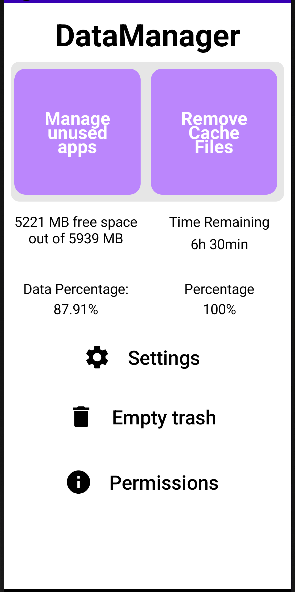
\includegraphics[width=200pt]{mainmenu.png}
    \caption{Main Menu Screen}
    \label{fig: Main Menu Screen}
\end{figure}

In Figure 5.1 we can see the main menu screen of the application, the user is greeted with a menu consisting of 5 buttons, each with its own unique functionality. The first time the user opens the application, some default settings will be placed and stored in the database, with the theme being a light one, the language being English, and no permissions being given by default, the app waiting for the user to give them when he either enters the cache screen and tries to analyze for residual files when he tries to enter the manage unused apps, or when he tries to press on the empty trash button. Each time the user tries one of these actions, the application will see if the permissions were granted, if so, the application can continue. 

\section{Permissions Menu}\label{sect:Permissions Menu}

\begin{figure}[htp]
    \centering
    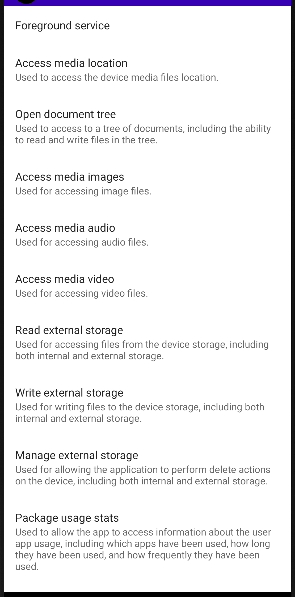
\includegraphics[width=200pt]{permissions.png}
    \caption{Permissions Menu Screen}
    \label{fig: Permissions Menu Screen}
\end{figure}

Figure 5.2 shows the screen that pops up when the user presses the permissions button in the main menu. The screen is used for telling the user what is he about to give his consent to, and what each of the required permissions is about. The permissions are as follows: 

    - Access media location;

    - Access foreground services;

    - Access image, video, and audio files;

    - Read both internal and external storage;

    - Write on both internal and external storage;

    - Manage both internal and external storage;

    - Package Usage stats, which allows the app to access information about the app usage;

    - Query all packages, which allows the app to gather information on all installed packages on the device;

\section{Settings Menu}\label{sect:Settings Menu}

\begin{figure}[htp]
    \centering
    \begin{minipage}{0.45\textwidth}
        \centering
        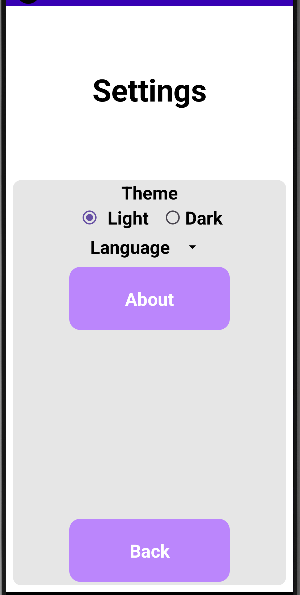
\includegraphics[width=205pt]{SettingsMenu.png}
        \caption{Light Settings Menu}
        \label{fig: Light Settings Menu}
    \end{minipage}\hfill
    \begin{minipage}{0.45\textwidth}
        \centering
        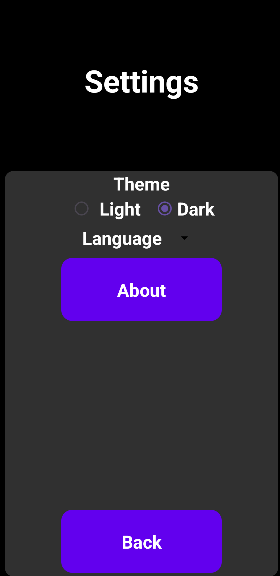
\includegraphics[width=200pt]{darksettingsmenu.png}
        \caption{Dark Settings Menu}
        \label{fig: Dark Settings Menu}
    \end{minipage}
\end{figure}
\newpage
Figures 5.3 and 5.4 showcase the settings menu and its buttons, those being the 2 radio buttons for the theme of the app, consisting of a Light and Dark mode, the Language dropdown menu used for changing the language of the application, the About button that opens the about menu which offers some additional information on what the app is about and the back button for going back to the main menu screen. The preferences set by the user are saved in the Firebase Realtime Database. 

The following 2 figures, Figures 5.5 and 5.6, showcase the changes in the layout of the application when the user chooses to change the language from English to Romanian, each element of text being changed to the other language seamlessly.

\begin{figure}[htp]
    \centering
    \begin{minipage}{0.45\textwidth}
        \centering
        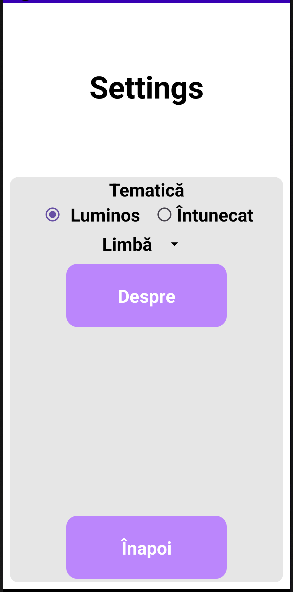
\includegraphics[width=205pt]{romanian.png}
        \caption{Settings Menu with Romanian text}
        \label{fig: Settings Menu with Romanian text}
    \end{minipage}\hfill
    \begin{minipage}{0.45\textwidth}
        \centering
        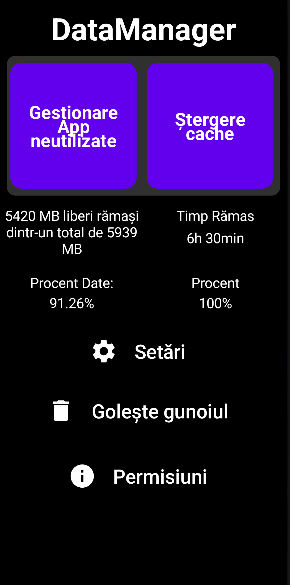
\includegraphics[width=200pt]{romanianmainmenu.png}
        \caption{Main Menu with Romanian text}
        \label{fig: Main Menu with Romanian text}
    \end{minipage}
\end{figure}
\newpage

\section{Cache Screen}\label{sect:Cache Screen}

\begin{figure}[htp]
    \centering
    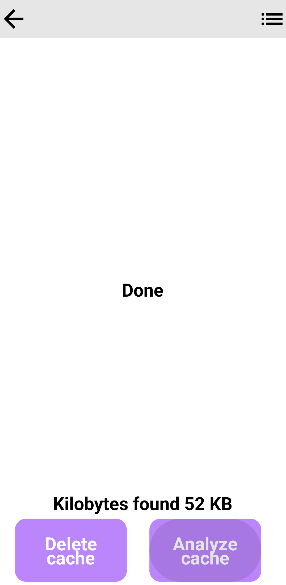
\includegraphics[width=200pt]{cachedeletionscreen.png}
    \caption{Cache Remover Screen}
    \label{fig: Cache Screen}
\end{figure}

Figure 5.7 showcases the Cache Deletion Screen. Here the user has several options, first, up top, is the back button on the top left, marked by a left-pointed arrow, and the second, top right, the filter settings, represented by the three lines, which, when pressed, takes the user to the filter settings of the app.

On the other hand, at the bottom, the other two buttons, analyze and delete, do pretty much what the name suggests, starting a general scan of the storage of the phone for signs of the type of files the user has selected, while the delete button removes said files. When clicking the buttons, a progress bar will appear showcasing that the search is still ongoing, and, after the search is done, 2 new texts appear, one saying "Done", and the other showcasing the amount of memory found/deleted.


\newpage
\begin{figure}[htp]
    \centering
    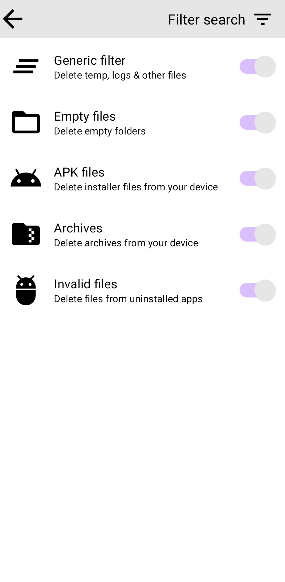
\includegraphics[width=200pt]{filter menu.png}
    \caption{File Filter Menu}
    \label{fig: File Filter Menu}
\end{figure}

The above figure, 5.8, presents the filter search settings menu that the app includes in the cache deleting screen. Here the user can switch on and off what type of files he or she wants to delete, those types ranging from temp, and logs to empty folders and leftover files, the screen shows for each file type a short description of what exactly the app will look for.

Each option is saved in a separate collection from the user preferences one, in Firebase Realtime Database, so that the user doesn't have to re-select what type of file he wants to get rid of each time they re-enters the application.

\newpage
\section{Unused App Screen}\label{sect:Unused App Screen}

\begin{figure}[htp]
    \centering
    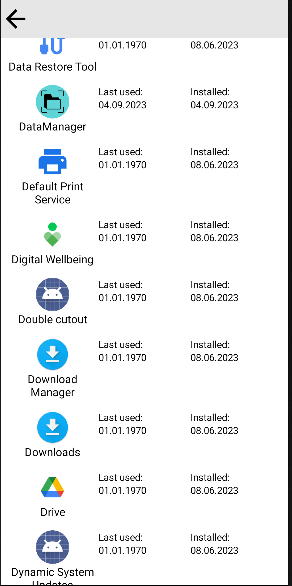
\includegraphics[width=200pt]{UnusedAppMenu.png}
    \caption{Unused App Menu}
    \label{fig: Unused App Menu}
\end{figure}

The Unused App Screen, shown in the 5.9 figure, lists all applications present in the users' application list, being ordered in an alphabetical manner. 

The list of applications showcases in three columns the name and icon, the last time they were used, and the date that the applications were installed. For applications that were never used or have been installed by default, usually, a generic date will be displayed, usually the Unix epoch, more specifically 1.01.1970, while apps that were actually used and installed by the user will showcase the correct dates.

\newpage
\begin{figure}[htp]
    \centering
    \includegraphics[width=200pt]{AppInfo.png}
    \caption{App Info}
    \label{fig: App Info}
\end{figure}

The user has the option in the Unused App Screen to click on any of the listed applications and be transported to the general App Info screen, as seen in the 5.10 figure. Here the user has the liberty to do whatever they want. It's up to them if they want to delete, force stop, set new preferences, and so on for the app they clicked on, or they can just as well leave it alone.

When done with the app, the user can go back to the DataManager app by simply clicking on the above arrow, the user being transported back to where they were on the app list.
\newpage
\begin{figure}[htp]
    \centering
    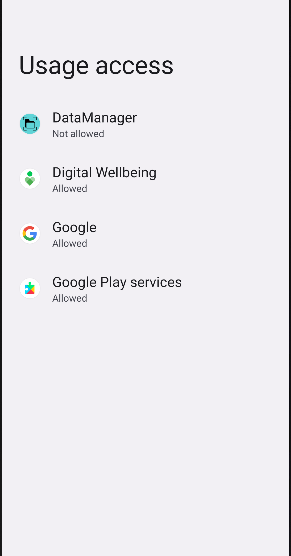
\includegraphics[width=200pt]{UsageAcess.png}
    \caption{Usage Access}
    \label{fig: Usage Access}
\end{figure}


The last figure, 5.11, represents the usage access screen that asks the user for the above-mentioned permissions, found in Figure 5.2. What the user needs to do here is simple, he needs to click on the DataManagerApp, and switch on the permission for usage access. 

After closing the usage access screen, another one will pop up that asks for access to all files in the system. Again, the user just has to click on the app, in the list, and check on the switch for storage permissions. After switching on the two options, the user will be able to use the functionalities of the application.
\newpage

%%%%%%%%%%%%%%%%%%%%%%%%%%%%%%%%%%%%%%%%%%%%%%%%%
%%%%%%%%%%%% chap: Conclusion %%%%%%%%%%%%%%%%%
%%%%%%%%%%%%%%%%%%%%%%%%%%%%%%%%%%%%%%%%%%%%%%%%%

\chapter{Conclusions \& Future work }\label{chapter:chap6}

\section{Conclusion}\label{sect:Conclusion}

In conclusion, the development of such applications represents an important step in the everyday user's ability to control and maintain their phones' storage and in keeping the phone clean of any unwanted data. Without such applications, most of us would be unaware of the reasons why our phones' storage capacity is being drained without our input. As such, the disadvantage of not being able to use our memory space however we want is diminished, leaving us with more freedom for how we use our phones.

This process of data cleaning can have lasting effects on the phone's life, most people not being aware of the fact that they can improve the lifespan of their phone by such methods. Too often one hears that people need to change their phone because it started to work slower, or that they need to buy one because they have too little memory left in it. With this in mind, making sure that our phone is well kept and once in a while cleaned is the same as cleaning our own homes, no one wants to live in a filthy house, so our phones should be treated with the same manner of respect.

\section{Future work}\label{sect:Future work}

Further improvements to applications such as this one are possible, ranging from data analysis over a set period of time to media optimization, such as the removal of duplicate image, audio, or video files, the management of notifications, application analysis, and so on.

Other areas that can be looked on are:

- Automation: We could look to improve the automation of data cleaning processes. This involves the development of new algorithms and techniques for automatically detecting errors in data. With the current \ac{AI} revolution, such automation processes could be the future of data-cleaning applications;

- The handling of complex data types: With data becoming more complex each passing day, there might come a growing need for data cleaning methods that can handle these types of complex data types and structures. 

\bibliography{mybib}
\bibliographystyle{alpha}
\addcontentsline{toc}{chapter}{Bibliography}

\end{document} 